\subsection{Single Qubit Readout on QICK System}
{{\footnotesize
\noindent Implements real-time ML models for single-qubit readout on the Quantum Instrumentation Control Kit (QICK), using hls4ml to deploy quantized neural networks on RFSoC FPGAs. Offers high-fidelity, low-latency quantum state discrimination. :contentReference[oaicite:0]\{index=0\}


\begin{description}[labelwidth=4cm, labelsep=1em, leftmargin=4cm, itemsep=0.1em, parsep=0em]
  \item[date:] 2025-01-24
  \item[version:] v1.0
  \item[last\_updated:] 2025-02
  \item[expired:] unknown
  \item[valid:] yes
  \item[valid\_date:] 2025-01-24
  \item[url:] \href{https://github.com/fastmachinelearning/ml-quantum-readout}{https://github.com/fastmachinelearning/ml-quantum-readout}
  \item[doi:] 10.48550/arXiv.2501.14663
  \item[domain:] Quantum Computing
  \item[focus:] Real-time single-qubit state classification using FPGA firmware
  \item[keywords:]
    - qubit readout
    - hls4ml
    - FPGA
    - QICK
  \item[licensing:] NA
  \item[task\_types:]
    - Classification
  \item[ai\_capability\_measured:]
    - Single-shot fidelity
    - inference latency
  \item[metrics:]
    - Accuracy
    - Latency
  \item[models:]
    - hls4ml quantized NN
  \item[ml\_motif:]
    - Real-time
  \item[type:] Benchmark
  \item[ml\_task:]
    - Supervised Learning
  \item[solutions:] Solution details are described in the referenced paper or repository.
  \item[notes:] Achieves \textasciitilde{}96\% fidelity with \textasciitilde{}32 ns latency and low FPGA resource utilization. 

  \item[contact.name:] Javier Campos, Giuseppe Di Guglielmo
  \item[contact.email:] unknown
  \item[datasets.links.name:] Zenodo: ml-quantum-readout dataset
  \item[datasets.links.url:] \href{zenodo.org/records/14427490}{zenodo.org/records/14427490}
  \item[results.links.name:] ChatGPT LLM
  \item[fair.reproducible:] Yes
  \item[fair.benchmark\_ready:] Yes
  \item[id:] single\_qubit\_readout\_on\_qick\_system
  \item[Citations:] \cite{diguglielmo2025endtoendworkflowmachinelearningbased}
\end{description}

{\bf Ratings:} ~ \\

\begin{tabular}{p{0.15\textwidth} p{0.07\textwidth} p{0.7\textwidth}}
\hline
Rating & Value & Reason \\
\hline
dataset & 4 & Dataset hosted on Zenodo with structured data; however, detailed documentation on
image acquisition and labeling pipeline is limited.
 \\
documentation & 4 & Codabench task page and GitHub repo provide descriptions and usage instructions,
but detailed API or deployment tutorials are limited.
 \\
metrics & 5 & Standard classification metrics (accuracy, latency) are used and directly relevant
to the quantum readout task.
 \\
reference\_solution & 1 & No baseline or starter models with runnable code are linked publicly.
 \\
software & 3 & Code and FPGA firmware available on GitHub; integration with hls4ml demonstrated.
Some deployment details and examples are provided but overall software maturity is moderate.
 \\
specification & 4 & Task clearly defined: real-time single-qubit state classification with latency and
fidelity constraints. Labeling and ground truth definitions could be more explicit.
 \\
\hline
\end{tabular}

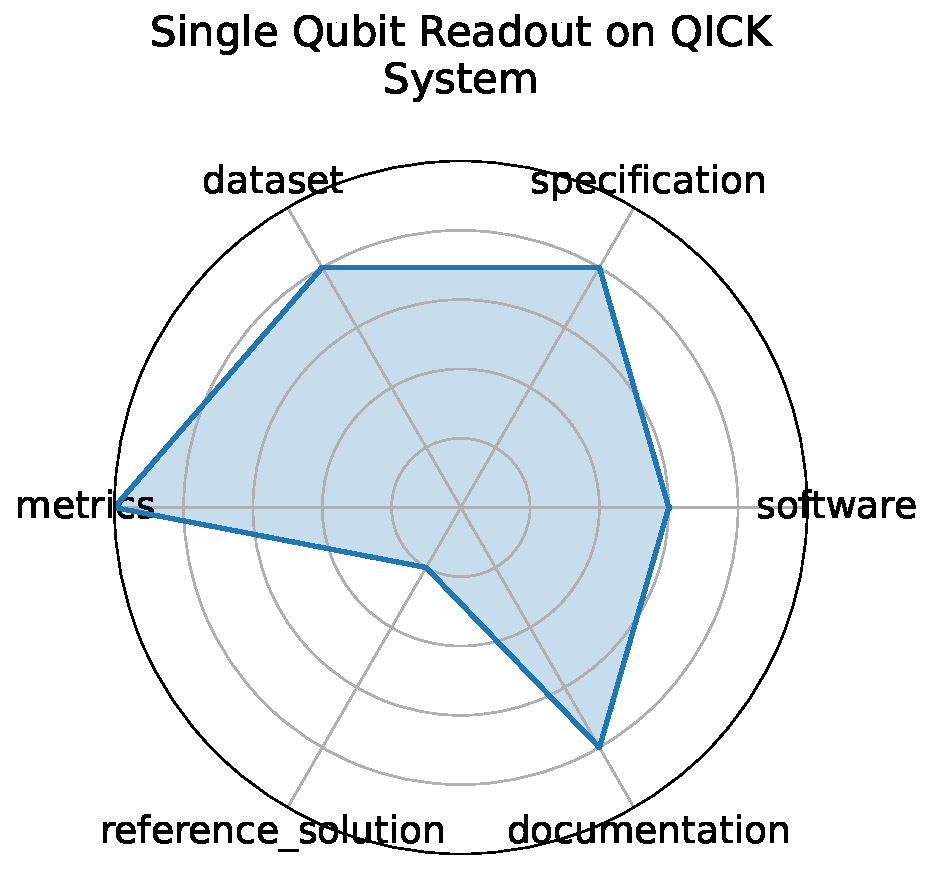
\includegraphics[width=0.2\textwidth]{single_qubit_readout_on_qick_system_radar.pdf}
}}
\clearpage